% vim: set spell spelllang=en_gb tw=80:
\chapter{Evaluation}\label{chapter:evaluation}

% \guidance{%
%   This is where Assessors will be looking for \textbf{signs of success} and for
%   \textbf{evidence of thorough and systematic testing}. \textbf{Sample output},
%   tables of timings and photographs of workstation screens, oscilloscope traces
%   or circuit boards may be included.\\
%   As with code, voluminous examples of sample output are usually best left to
%   appendices or omitted altogether.\\
%   There are some obvious questions which this chapter will address. \textbf{How
%   many of the original goals were achieved? Were they proved to have been
%   achieved? Did the program, hardware, or theory really work?}\\
%   Assessors are well aware that large programs will very likely include some
%   residual bugs. It should always be possible to demonstrate that a
%   \textbf{program works in simple cases} and it is instructive to
%   \textbf{demonstrate how close it is to working in a really ambitious case}.\\
% }

\prechapter{%
  In this chapter, I will show that the project meets its aims (as listed in
  Section~\ref{intro:aims}) by presenting the evidence for this claim. I will
  do so by (a) comparing the project with existing tools that aim to help a
  user understand a Coq library and (b) providing sample output and explaining
  the insights they provide.
}%

\section{Features}\label{eval:compare}

I talked through most of the first aim (how I represent Coq libraries as Neo4j
databases) in the~\nameref{chap:impl} chapter. To assess the capabilities of my
project, and thereby the suitability of my chosen model, I will compare all the
programs listed in Subsection~\ref{prep:coqtools},~\nameref{prep:coqtools} with
this project against the features listed there (features chosen to reflect
strengths of each tool considered).

The project \emph{can be extended} to support \textbf{linking to source code}
by modifying either the model, database or JavaScript visualisations (output
by the library of queries) to link to the relevant webpages output by coqdoc.
So, a user could switch between a graphical overview and a detailed inspection
at will.

Whenever a node is visible, it can be expanded to see the nodes it depends on,
so in that sense, it supports \textbf{hyperlinks}, though, unlike hyperlinks,
such expansion is done in place, thus retaining the \emph{context} of its use.

Thanks to the \emph{kind} and \emph{subkind} labels, the project supports
\textbf{precise kinds}.  Also, any (co-)inductive \textbf{type} can, via the
\texttt{CONSTRUCTED\_BY} relation, be expanded to see its
\textbf{constructors}.

Due to the type property, each object's \textbf{type-signature} is also visible.
Crucially, it is a fully-expanded type-signature, making explicit any
assumptions introduced (perhaps hundreds of lines prior or in a different file)
into the environment.

\textbf{Module dependencies} are set with the query in Listing~\ref{lst:moddep}
using the \texttt{CONTAINS} relation. \textbf{Interactivity} is achieved through
the Neo4j browser interface and the JavaScript visualisations;
\textbf{statistics} are achieved through the library of queries;
\textbf{graphical representations} by both.

An important limitation of CoqSerAPI is that its \textbf{statistics} are (at
the time of writing) simply three counters, whereas this project offers many
sophisticated graph metrics and the ability (through a queriable database) to
gain \emph{any} sort of information a user is interested in.

\begin{listing}[tp]%

\caption{Query to set Module Dependencies}\label{lst:moddep}

  \begin{minted}{cypher}
    MATCH (a)-[:USES]->(b),
          (src:module)-[:CONTAINS]->(a),
          (dst:module)-[:CONTAINS]->(b)
    WHERE src.objectId <> dst.objectId
    CREATE UNIQUE (src)-[r:DEPENDS_ON]->(dst)
    SET r.weight = coalesce(r.weight, 0) + 1
    RETURN r
  \end{minted}

\end{listing}

And finally, \textbf{object dependencies} are at the heart of the project: by
using a Neo4j graph database, a user can understand and manipulate this
relation in a much more flexible and scalable manner than any visualisation can
manage.

Therefore, the project either supports, or can be extended to support, every
feature supported by other tools.  This project also supports additional
features not in other tools: structural queries, network-analysis algorithms and
visualisations.

\section{Performance}

Now, I will compare the project's execution time to most of the tools from the
previous section. This project is slightly slower than other tools because it
has more features and is more flexible.

\subsection{Setup}

To evaluate timings, I used the Coq (8.6) Standard Library, due to its sheer
size (564 modules, 5823 definitions, 23,892 proofs). For coqdoc and coqdep, I
modified Coq's Makefiles to measure execution time using bash's \emph{time}
command. At the time of writing, CoqSerAPI's statistics were not fully/usably
implemented, so I did not include it in this comparison. For dpdgraph, I took
separate measurements for outputting a \texttt{.dpd} file and converting that
file to a \texttt{.dot} format. I took a similar approach for this project, so
that the comparison was as fair as possible.

\begin{figure}[tp]
\centering
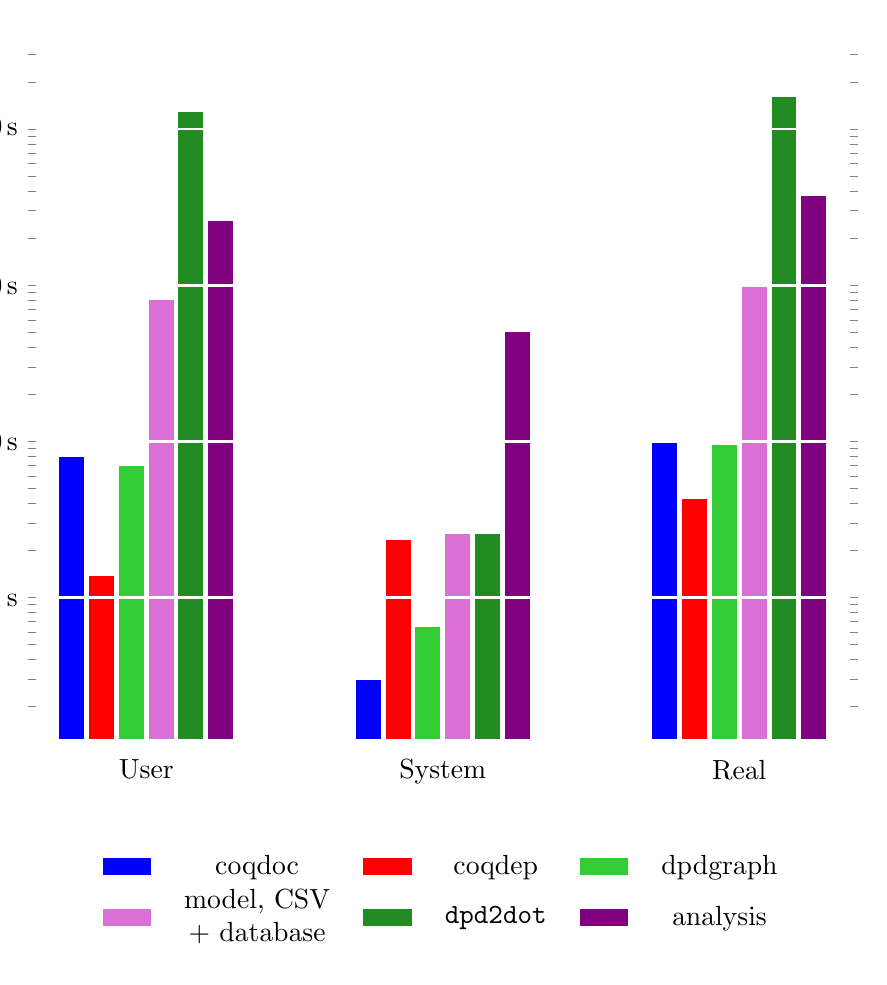
\begin{tikzpicture}[trim axis left]
	\begin{axis}[
    % width of chart
    width=\textwidth,
    % no box, below chart, horizontal
		legend style={%
      draw=none,
      at={(0.5,-0.15)},
      anchor=north,
      legend columns=3,
      column sep = 1em,
      cells={align=center},
    },
    % value above position on bar chart
		ybar=0.5ex, % bar chart, with inter-bar spacing of 1ex
    log ticks with fixed point,
    yticklabel={\pgfmathparse{pow(10,\tick-3)}\pgfmathprintnumber[fixed]{\pgfmathresult}}\,s, % N ms along y-axis
    symbolic x coords={User,System,Real},
		xtick=data,
    axis line style={opacity=0}, % hide y axis
    major tick style={draw=none}, % no ticks
    ymode=log, % log scale for y
    log basis y = {10}, % log base 10
		enlarge x limits=0.20, % spacing on x axis
    bar width=2ex,
    ymajorgrids, % rows of lines
    major grid style={white, line width=1pt},
    axis on top,
	]

  % Coqdoc
  \addplot [area legend, style={Blue,fill=Blue,mark=none}]
    coordinates {(User,7877) (System,0295) (Real,10007)};

  % Coqdep
  \addplot [area legend, style={red,fill=red,mark=none}]
    coordinates {(User,1361) (System,2299) (Real,4257)};

  % dpdgraph
  \addplot [area legend, style={LimeGreen,fill=LimeGreen,mark=none}]
    coordinates {(User,6872) (System,0645) (Real,9392)};

  % creation
  \addplot [area legend, style={Orchid,fill=Orchid,mark=none}]
    coordinates {(User,79254) (System,2521) (Real,98157)};

  % dpd2dot
  \addplot [area legend, style={ForestGreen,fill=ForestGreen,mark=none}]
    coordinates {(User,1272249) (System,2516) (Real,1588303)};

  % analysis
  \addplot [area legend, style={violet,fill=violet,mark=none}]
    coordinates {(User,255912) (System,49569) (Real,371881)};

  \legend{coqdoc,coqdep,dpdgraph,{model, CSV\\+ database},\texttt{dpd2dot},analysis}

	\end{axis}

\end{tikzpicture}

\caption{Comparison of Execution Times. Note that the data is presented on a
  \emph{logarithmic} scale. We see coqdoc takes very little time to run, and
  coqdep even less (which is to be expected considering their purely lexical
  approach). Somewhat surprisingly, dpdgraph runs just as quickly as coqdoc;
  its increase in system time can be explained by the 14MB \texttt{dpd} file
  output by dpdgraph. Although at first it appears that there is an
  order-of-magnitude slowdown with this project, more detailed examination in
  Subsection~\ref{subsec:ineff} explains precisely \emph{what} occurs during
  database creation and where inefficiencies lie.}\label{fig:exectimes}
\end{figure}

\subsection{Inefficiencies}\label{subsec:ineff}

Setting up a graph database from scratch can take some time. Assuming a Coq
project is already compiled, the following steps need to take place:

\begin{enumerate}
  \item\label{step:gen} generating file with a list of all the modules to be
    examined (15 ms),
  \item\label{step:compile} compile that file using the Coq compiler (12.6 s),
  \item\label{step:dpd2csv} convert the output \texttt{.dpd} file to CSV files (72.7 s),
  \item create a Neo4j database from those CSV files (12.8 s)
\end{enumerate}

When steps~\ref{step:gen} and~\ref{step:compile} are taken on their own, we see
that the changes to accommodate a more detailed model resulted in a 25\%
slowdown, which is acceptable given this is a stress-test and the difference is
on the order of seconds. Creating a database from CSV files takes a similar
amount of time, also acceptable given the size of the graph (31,088 nodes and
850,434 edges).

So, the real bottleneck is step~\ref{step:dpd2csv}: converting \texttt{.dpd}
files to CSV. During execution, \texttt{dpd2} reads in a 25MB \texttt{.dpd} file
and outputs two CSV files of size 7MB (nodes) and 8MB (edges), so IO is likely
to be a factor, as is reconstructing the graph in memory. I output the model to
a \texttt{.dpd} to make it easier to extend this project with other tools. It is
likely that outputting a CSV directly would have resulted in being able to
bypass this phase altogether, but from a software-engineering point-of-view, the
trade-off there is increased coupling for faster execution.

\subsection{Graph Analysis \& Visualisation}

Once a graph is created (whether it be in the form of \texttt{.dpd} file or a
database) the last step is to \emph{use} the data by analysing and visualising
it. Here, this project shows a significant improvement over \texttt{dpd2dot}.

At nearly \emph{27 minutes}, its execution time dwarfs the analyses carried out
by this project. Whereas \texttt{dpd2dot} converted the output 13MB
\texttt{.dpd} file to a 24MB dot file, in about one-quarter of the time, an R
script could run (a) PageRank and closeness centrality algorithms over all
proofs and definitions and (b) output \emph{8} different 9MB visualisations of
the data. Analyses took less than a minute; visualisations ranged from 20 to 90
seconds.

It should be noted that \texttt{dpd2dot} does not do graph \emph{layout}: it
just splits the graph into sub-graphs (based on modules) and assigns a colour
and label to each node (based on their properties). Converting the
\texttt{.dot} file to a viewable format (e.g.\ a scalable vector-graphic or
SVG) is up to another tool (that being said, I cancelled the command
\texttt{dot -Tsvg} to produce an SVG after it failed terminate within a few
\emph{hours}).

\section{Library of Queries}\label{sec:libeval}

I talked through how I provide several-network analysis techniques in
the~\nameref{chap:impl} chapter. To assess whether this tool highlights the
structure of and relationship between proof-objects (the second aim), I will
show the output of the library of queries on the small case of a Coq
Regular-Expression library and on the large case of the project's moon-shot, the
Odd Order Theorem.

\emph{All} visualisations (except Figure~\ref{fig:regexp:meta}) show only
definitions (shown as triangles, reminiscent of the $\triangleq$ symbol
sometimes used for definitions) and proofs (shown as squares, reminiscent of the
end-of-proof $\square$ symbol), except for Figures~\ref{fig:regexp:module},
\ref{fig:oot:module} and~\ref{fig:oot:modhier} which also include modules (as
circles).

\subsection{Small: CoqRegExp}

I will now show, how, without studying any code, a Coq user can use this
project to understand the structure of the CoqRegExp library.

\subsubsection{Neo4j \& APOC}

As visible by the examples in Tables~\ref{table:regexp:kinds}
and~\ref{table:regexp:pagerank}, and Figure~\ref{fig:regexp:meta}, a user can
make arbitrary queries on the CoqRegExp library database. The first gives an
indication of the most common kinds of proof-objects: mostly lemmas, with
definitions and proofs following.  The second uses an APOC procedure for
PageRank over all proof-objects to quantify the importance of each. The
definition of a regular-expression and the definition of what it means for a
regular-expression to match a string top the table, with other, fundamental
theory components/proof-objects following. The third also uses an APOC
procedure to produce a visual representation of the schema of the database.

\begin{table}[tp]
  %TC:ignore
\begin{minted}{cypher}
MATCH (obj) RETURN LABELS(obj), count(*) AS total
ORDER BY total DESC LIMIT 5
\end{minted}
%TC:endignore

\centering

\begin{tabular*}{\textwidth}{@{\extracolsep{\fill}} lc}

  \toprule
  \textbf{LABELS(obj)} & \textbf{total} \\

  \midrule

  proof, lemma         & 79 \\
  definition           & 17 \\
  proof, theorem       & 16 \\
  definition, instance & 14 \\
  type\_constructor    & 8 \\

  \bottomrule

\end{tabular*}

\bigskip
\caption{Top 5, most common kinds of proof-objects in CoqRegExp with their
  frequency and the query used to obtain them above the
  table.}\label{table:regexp:kinds}

\end{table}

\begin{table}[tp]
  %TC:ignore
\begin{minted}{cypher}
MATCH (n) WITH collect(n) AS nodes
CALL apoc.algo.pageRank(nodes) YIELD node, score
RETURN node.name, LABELS(node), node.path, score
ORDER BY score DESC LIMIT 5
\end{minted}
%TC:endignore

\centering

\begin{tabular*}{\textwidth}{@{\extracolsep{\fill}} lllc}

  \toprule
 \textbf{node.name} & \textbf{node.path} & \textbf{LABELS(node)} & \textbf{score} \\

  \midrule

  RegExp   & RegExp.Definitions & inductive\_type, inductive & 7.12518 \\
  matches  & RegExp.Definitions & definition, fixpoint       & 3.12445 \\
  Or       & RegExp.Definitions & type\_constructor          & 2.35997 \\
  re\_eq   & RegExp.Definitions & definition                 & 2.30212 \\
  Cat      & RegExp.Definitions & type\_constructor          & 2.04202 \\

  \bottomrule

\end{tabular*}

\bigskip
\caption{Top 5 proof-objects by PageRank in CoqRegExp, with the modules they
  are in, their kinds, their PageRank values, and the query used to
  obtain them above the table.}\label{table:regexp:pagerank}

\end{table}

\begin{figure}[tp]
\begin{minted}{cypher}
CALL apoc.meta.graph
\end{minted}
\centering
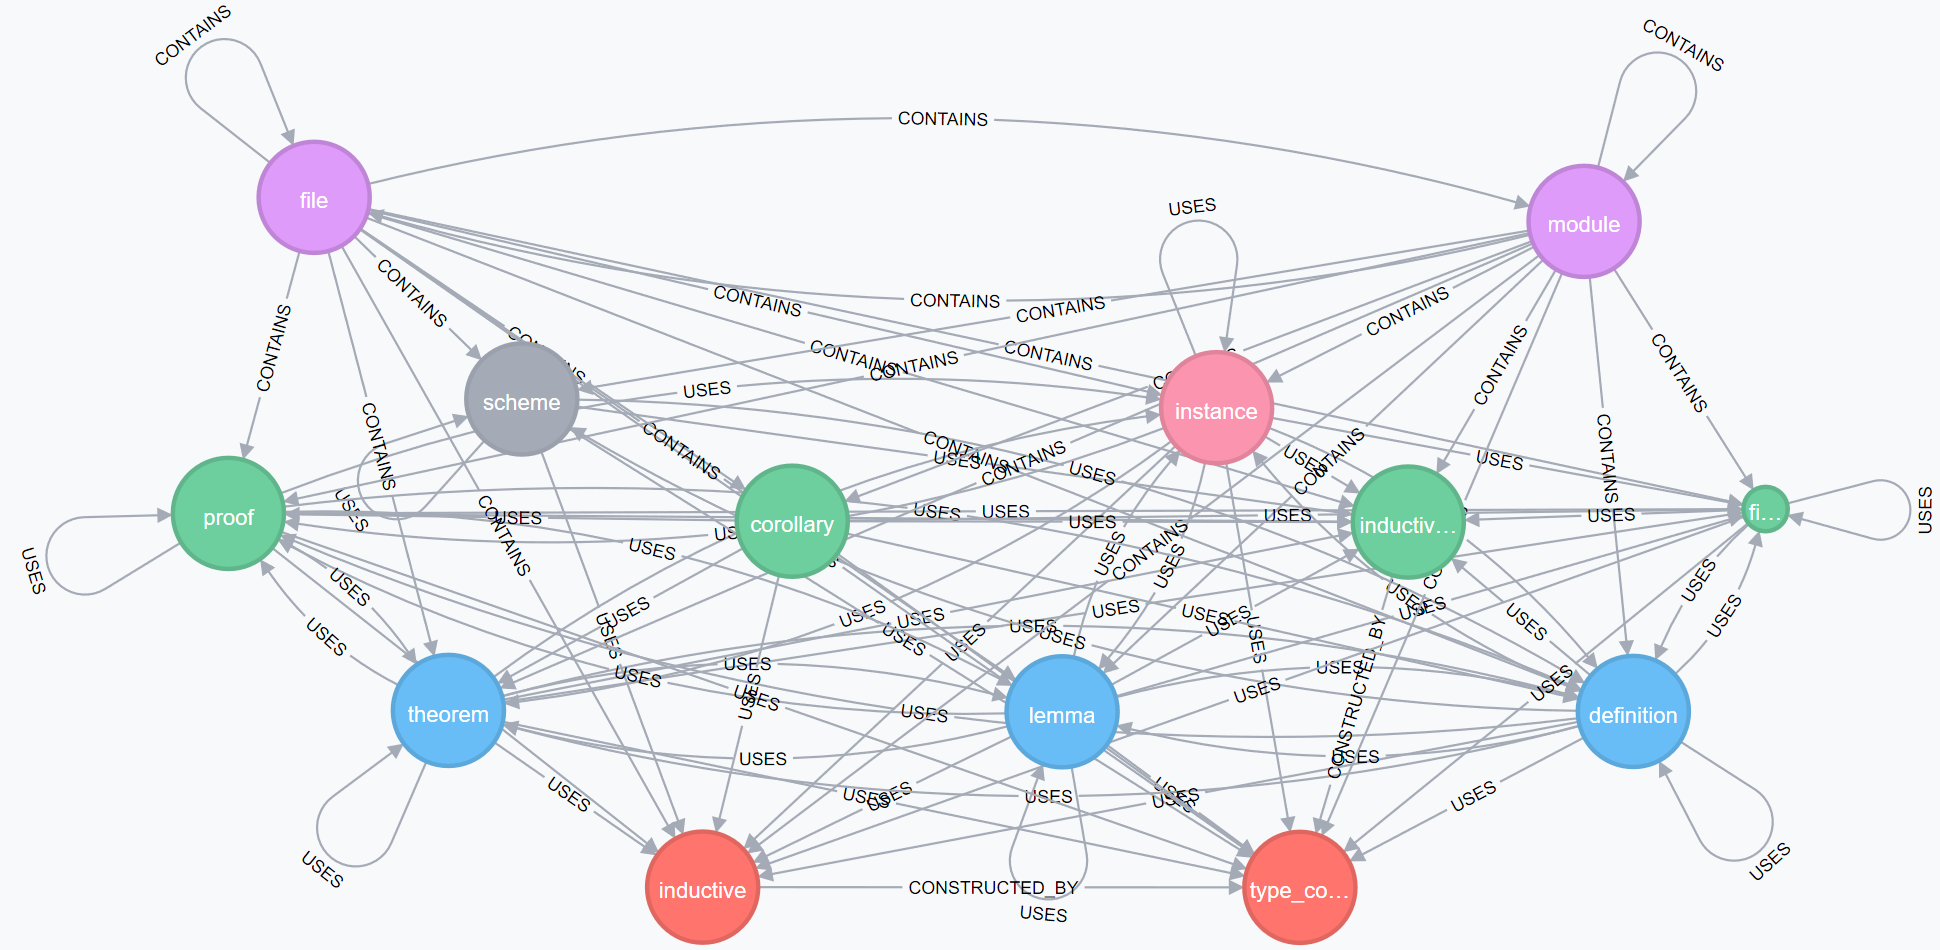
\includegraphics[width=\textwidth]{img/regexp/meta.png}
\caption{Meta-graph of CoqRegExp representing the labels (kinds/subkinds) and
  relations (\texttt{USES}, \texttt{CONTAINS}, \texttt{CONSTRUCTED\_BY})
  between them. Above the figure is the Cypher query which calls the APOC
  procedure to produce this. At the bottom, red nodes represent types and
  constructors; above them, blue nodes represent definitions; above them, green
  nodes represent proofs. The grey node represents a scheme; the pink node
  represents an instance and the two purple nodes at the top represent files
  and modules.}\label{fig:regexp:meta}
\end{figure}

\subsubsection{Visualisation}\label{subsubsec:visualisation}

Intuitively, in Figures~\ref{fig:regexp:direct} and~\ref{fig:regexp:module},
the \glblue{light blue} cluster represents \glblue{\emph{executable
functions}}; the \gorange{orange} cluster represents \gorange{\emph{proofs of
correctness}}; the \glpurple{light purple} cluster represents proofs using the
definition of \glpurple{string length}; the \glgreen{light green} cluster
represents proofs involving \glgreen{converting strings to
regular-expressions}; the \gviolet{violet} cluster represents proofs related
to \gviolet{nullable strings}. The node at the centre of the \glblue{light
blue} cluster is a function which computes whether a given regular-expression
matches a given string; the node at the centre of the \gorange{orange} cluster
defines what it means for two regular-expressions to be equal.

\begin{figure}[tp]
\centering
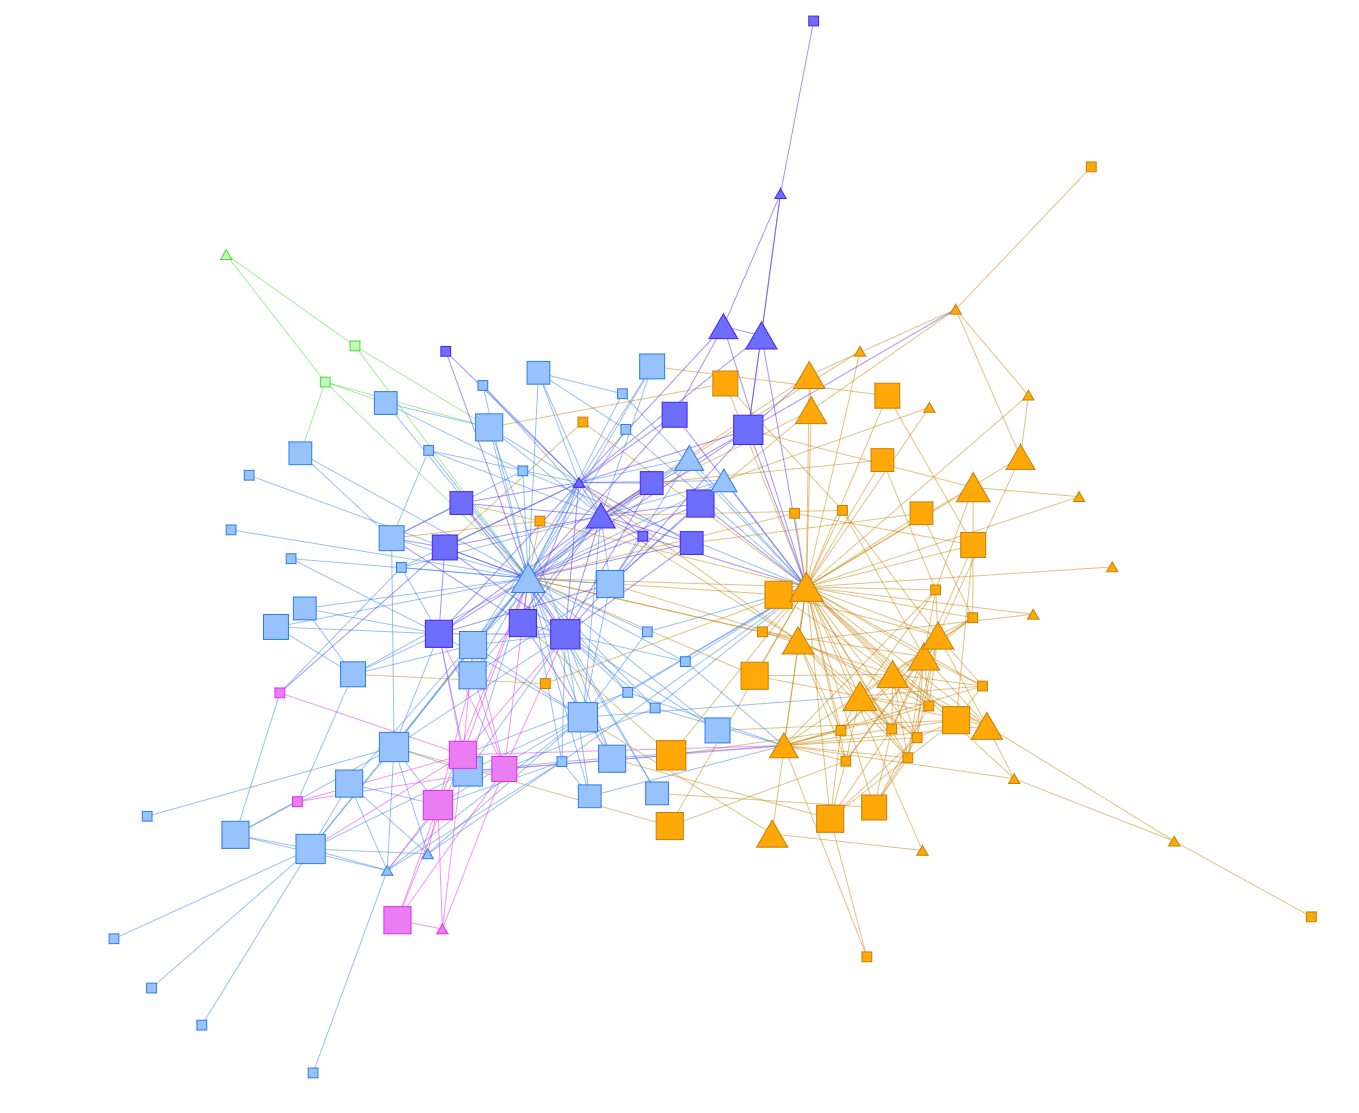
\includegraphics[height=0.3\textheight]{img/regexp/direct.png}
\caption{Force-directed visualisation of definitions and proofs in CoqRegExp.
  Colours assigned by modularity clustering largely correspond to the how a
  human might group nodes visually: two major clusters with a few, smaller
  clusters (see~\ref{subsubsec:visualisation}~\nameref{subsubsec:visualisation}
  for an interpretation of what each colour corresponds to). The size of the
  nodes corresponds to betweenness centrality scores (split up into 10
  logarithmically equal-width buckets). Edges represent the \texttt{USES}
  relation; edge-directions (source-uses-destination) are omitted for clarity
  since they generally point toward the centre of a
  cluster.}\label{fig:regexp:direct}
\end{figure}

\begin{figure}[tp]
\centering
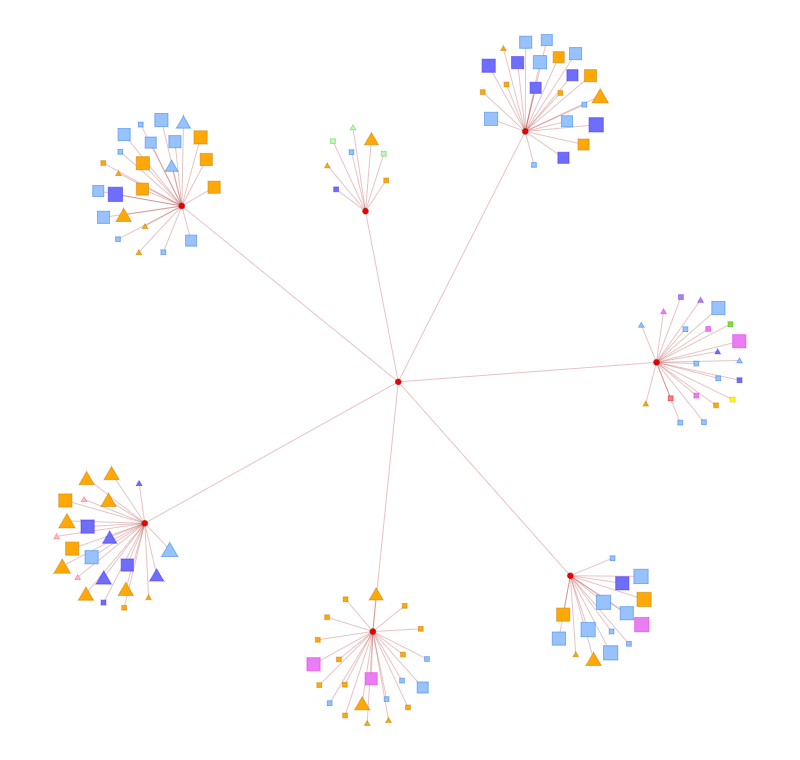
\includegraphics[height=0.3\textheight]{img/regexp/module.png}
\caption{Force-directed visualisation of definitions, proofs and modules in
  CoqRegExp. Setup is like Figure~\ref{fig:regexp:direct} above, except
  edges represent the \texttt{CONTAINS} relation. Each module tends to have two
  main parts: those relating to \glblue{executable functions} those relating to
  \gorange{proofs of correctness}, occasionally accompanied by a few
  definitions/proofs on \gviolet{nullability} or \glpurple{string
  length}.}\label{fig:regexp:module}
\end{figure}

\subsection{Large: Odd Order Theorem}

This Coq library closely follows the structure of the source material it
encodes: Peterfalvi~\cite{peterfalvi2000oot} and Bender \&
Glauberman~\cite{bender1994oot}. Each section (chapter) in the original books is
a file/module in the Coq library; each definition/lemma/corollary/etc.\
corresponds to the same in the books. Following the convention in the Coq
library, `Bender \& Glauberman' will henceforth be abbreviated to `BG' and
`Peterfalvi' to `PF'. For brevity, `Odd Order Theorem' will also be abbreviated,
to `OOT'.

I will now show, how, without studying any code, or reading BG or PF, a Coq user
can use this project to understand the structure of BG and PF.

New to this section, edges are coloured. Unless a figure is stated as being
`flipped', the colour of an edge is the same colour as its source (user);
otherwise, it is the same colour as its destination (used).

\subsubsection{Neo4j}

By modelling Coq libraries as Neo4j graph databases, we can answer powerful
questions. For example: there are 1064 proofs in BG and PF, \emph{does every
one of them ultimately lead to the proof of the Feit-Thompson OOT?} In
general, how many ``dead-ends'' -- proofs, definitions or types -- are there
in these two books, and where are they? These questions have been answered in
Tables~\ref{table:oot:leadto} and~\ref{table:oot:unused} respectively.

\begin{table}[tp]
  \begin{minted}{cypher}
MATCH (q:proof) 
WHERE NOT (:proof {path: "mathcomp.odd_order.PFsection14",
                   name : "Feit_Thompson"})
          -[:USES*]->(q:proof)
RETURN q.name, replace(q.path, "mathcomp.odd_order.", "") AS path
\end{minted}

\centering

\begin{tabular*}{\textwidth}{@{\extracolsep{\fill}} ll}

  \toprule

	\textbf{q.name}	& \textbf{path} \\

	\midrule

	pcore\_Fcore     & BGsection15 \\
	main            & stripped\_odd\_order\_theorem\ldots\\
	ell\_sigma\_leq\_2 & BGsection14 \\
	Ptype\_trans     & BGsection14 \\
	P1type\_trans    & BGsection14 \\

  \bottomrule

\end{tabular*}

\bigskip
\caption{Five (of 89), proofs the Odd Order Theorem Coq library which do not
  ultimately lead to the proof of the Feit-Thompson Odd Order Theorem. Module
  names (path property) have been shortened to remove redundant
  information. The ``stripped\_odd\_order\_theorem'' is a self-contained proof
  relying on only basic Coq features and is not part of BG or
  PF.}\label{table:oot:leadto}

\end{table}

\begin{table}[tp]
  \begin{minted}{cypher}
MATCH (q) WHERE NOT((q:module) OR ()-[:USES]->(q))
RETURN LABELS(q),
       REPLACE(q.path, "mathcomp.odd_order.", "") AS path, 
       COUNT(*) AS total
ORDER BY total DESC LIMIT 7
\end{minted}

\centering

\begin{tabular*}{\textwidth}{@{\extracolsep{\fill}} llc}

  \toprule

  \textbf{LABELS(q)} & \textbf{path} & \textbf{total} \\

  \midrule

  definition, scheme & stripped\_odd\_order\_theorem & 27 \\
  proof, lemma       & BGsection16                   & 6 \\
  proof, lemma       & BGsection15                   & 5 \\
  proof, lemma       & PFsection8                    & 5 \\
  proof, lemma       & BGsection10                   & 4 \\
  proof, remark      & BGsection14                   & 4 \\
  proof, lemma       & PFsection5                    & 4 \\

  \bottomrule

\end{tabular*}

\bigskip
\caption{Top 7 kinds of proof-objects in the OOT Coq library which are never
  used again (of which there are 107), grouped by module and ordered by
  frequency.  Module names (the `path' property) have been shortened to remove
  redundant information. The `stripped\_odd\_order\_theorem' is a
  self-contained proof of the entire OOT relying only on basic Coq features and
  is not part of BG or PF. Many unused results are simply called `lemma'
  instead of the more descriptive and conventional `corollary' or
  `remark'.}\label{table:oot:unused}

\end{table}

\subsubsection{Visualisation}\label{subsubsec:oot:visual}

In Figure~\ref{fig:oot:direct}, we see that modularity clustering over proofs
and definitions connected by the \texttt{USES} relation distinguishes
\emph{more} groups than force-directed visualisation does, despite appearing to
be a highly interconnected theory.

% Direct
\begin{figure}[tp]
\centering
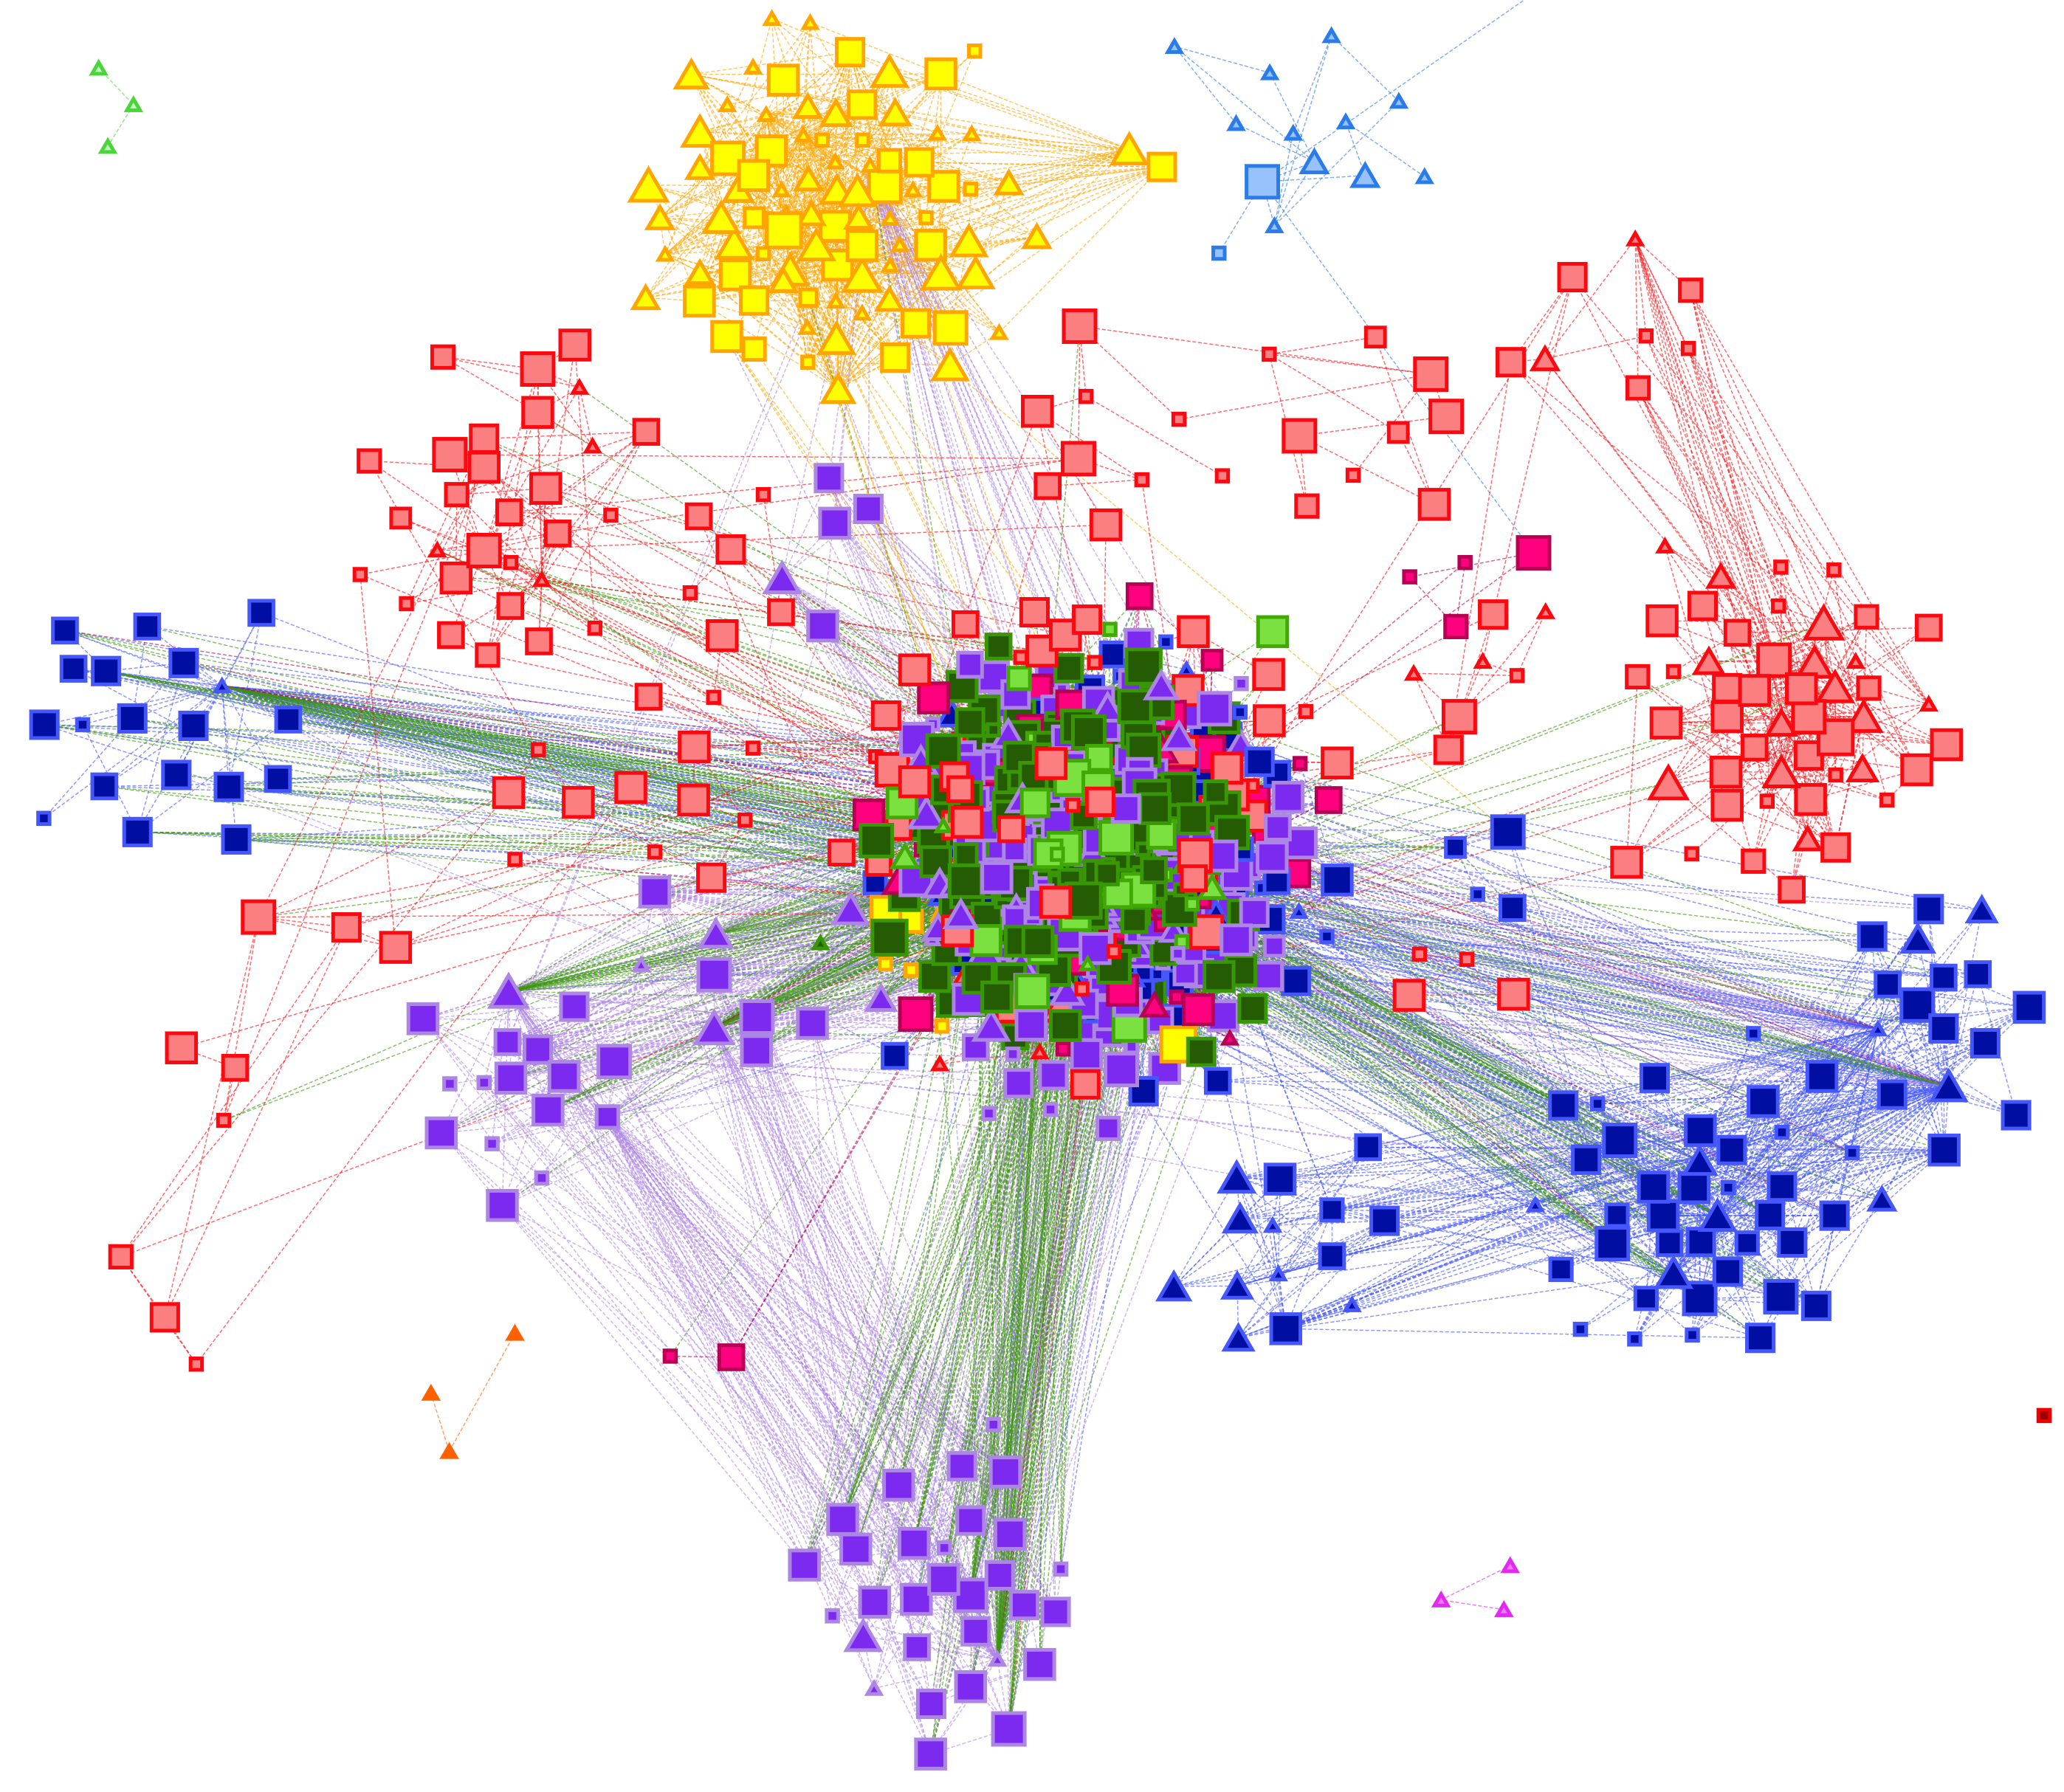
\includegraphics[height=0.35\textheight]{img/oot/direct}
\caption{Force-directed visualisation of definitions and proofs in the OOT Coq
  library (some nodes omitted for clarity). Setup is the same as that of
  Figure~\ref{fig:regexp:direct}. Observe that modularity clustering can
  distinguish between nodes in the centre as belonging to different groups. This
  distinction is more evident in Figures~\ref{fig:oot:module},
  \ref{fig:oot:modhier}, \ref{fig:oot:hier}
  and~\ref{fig:oot:hierflip}; it is explained in
  \ref{subsubsec:oot:visual}~\nameref{subsubsec:oot:visual}.}\label{fig:oot:direct}
\end{figure}

Figure~\ref{fig:oot:module} shows visually what one might expect intuitively:
\emph{proofs and definitions within the same module tend to belong to the same
group}. It explains why modularity clustering could distinguish more groups than
force-directed visualisation could. However, it does not explain why the groups
\emph{cross} module boundaries and represent \emph{multiple} modules.

% Modules
\begin{figure}[tp]
\centering
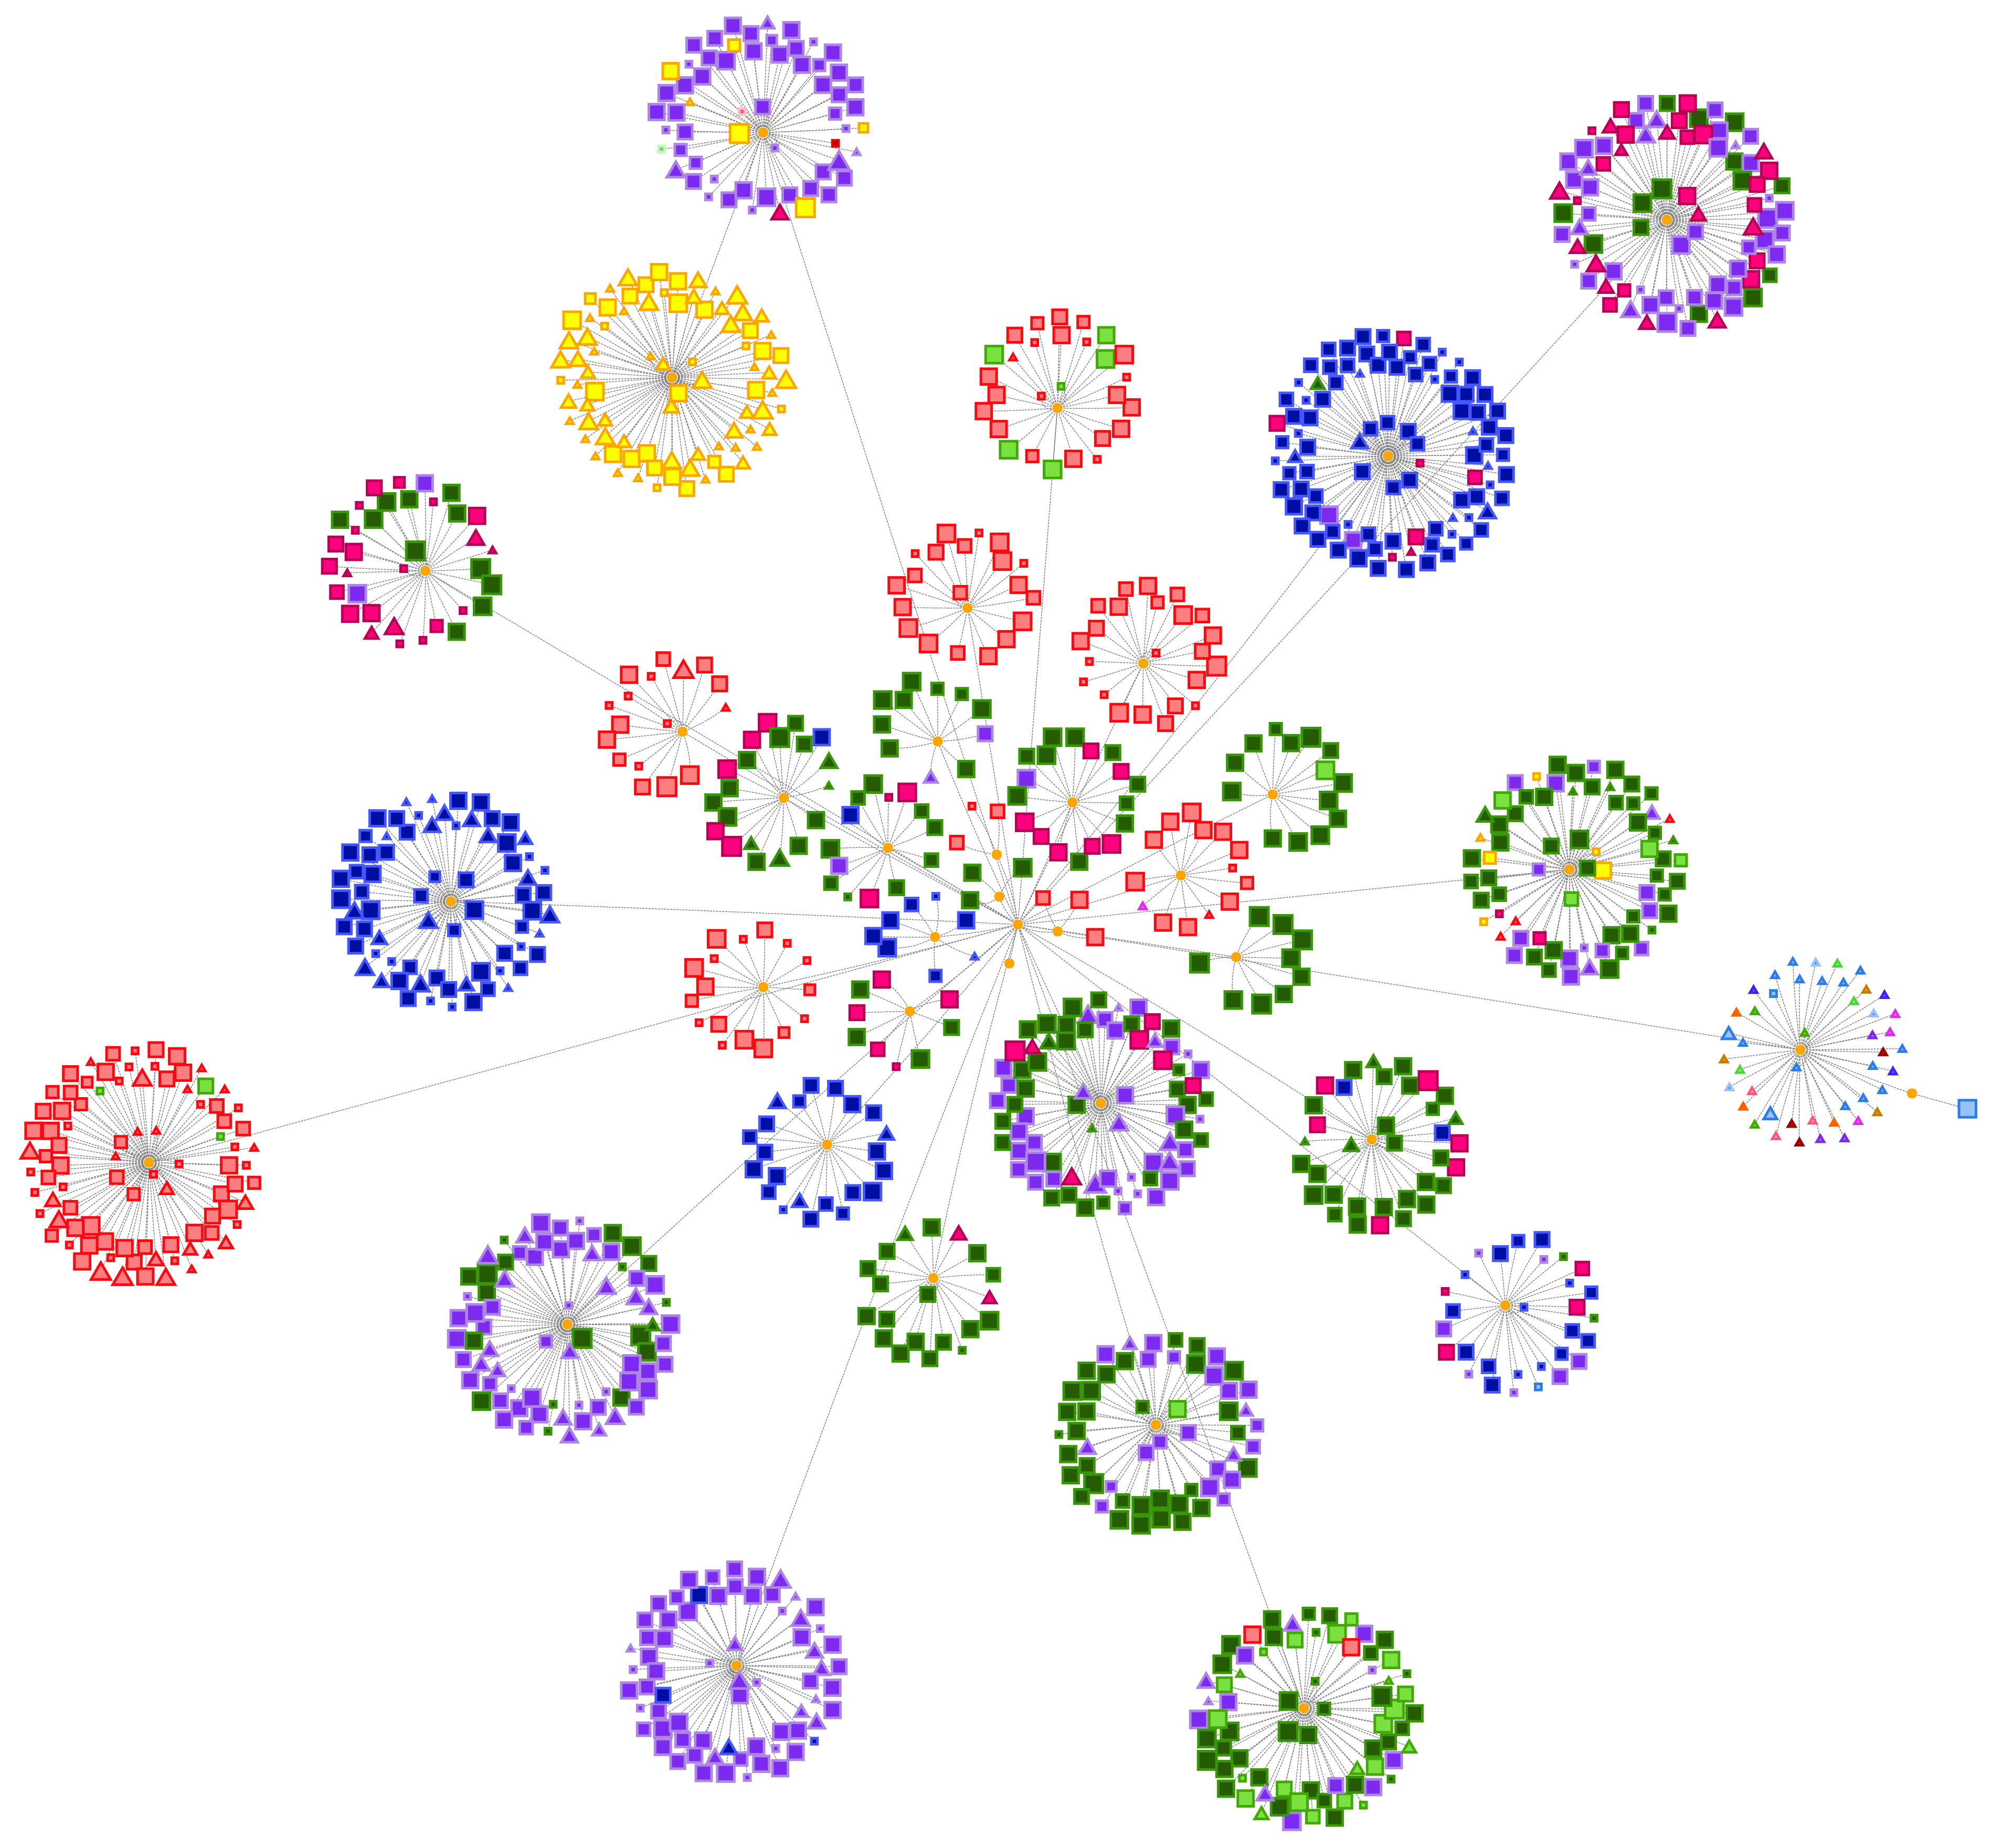
\includegraphics[height=0.35\textheight]{img/oot/modules}
\caption{Force-directed visualisation of definitions, proofs and modules in
  the OOT Coq library. Setup is the same as that of
  Figure~\ref{fig:regexp:module}. The module in \gyellow{yellow} --
  a self-contained result by the name of `CyclicTIisoReflexion' -- is
  the only one \emph{nested} inside another (PF~3). Unlike CoqRegExp, here,
  proofs and definitions in each module tend to belong to the same group. Note
  that groupings \emph{cross} module boundaries; this is elaborated upon in
  \ref{subsubsec:oot:visual}~\nameref{subsubsec:oot:visual}.}\label{fig:oot:module}
\end{figure}

Figure~\ref{fig:oot:modhier} explains why the groups cross module boundaries:
they demarcate different parts/phases of BG and PF. Both the figure and the list
below show this Coq library is not quite the linear chain of dependencies ranges
one may expect. Instead, the overlapping ranges of these groups suggest that the
material is heavily interconnected and that there are other ways of approaching
the material other the linear presentation of BG and PF.

\begin{itemize}
  \item \gpink{\textbf{pink:}  BG 1-6 and BG Appendices A/B/C}
  \item \gdgreen{\textbf{dark green:} BG 7-13 and PF 9-10 and 12-14}
  \item \gpurple{\textbf{purple:} BG 14/16 and PF 3-4/8}
  \item \gyellow{\textbf{yellow:} CyclicTIisoReflexion in PF 3}
  \item \gmagenta{\textbf{magenta:} BG 15 and PF 11}
  \item \gdblue{\textbf{dark blue:} PF 1-2 and 5-7.}
  \item \glblue{\textbf{light blue:} self-contained proof of the OOT.}
\end{itemize}

% Hierarchical Modules
\begin{figure}[tp]
\centering
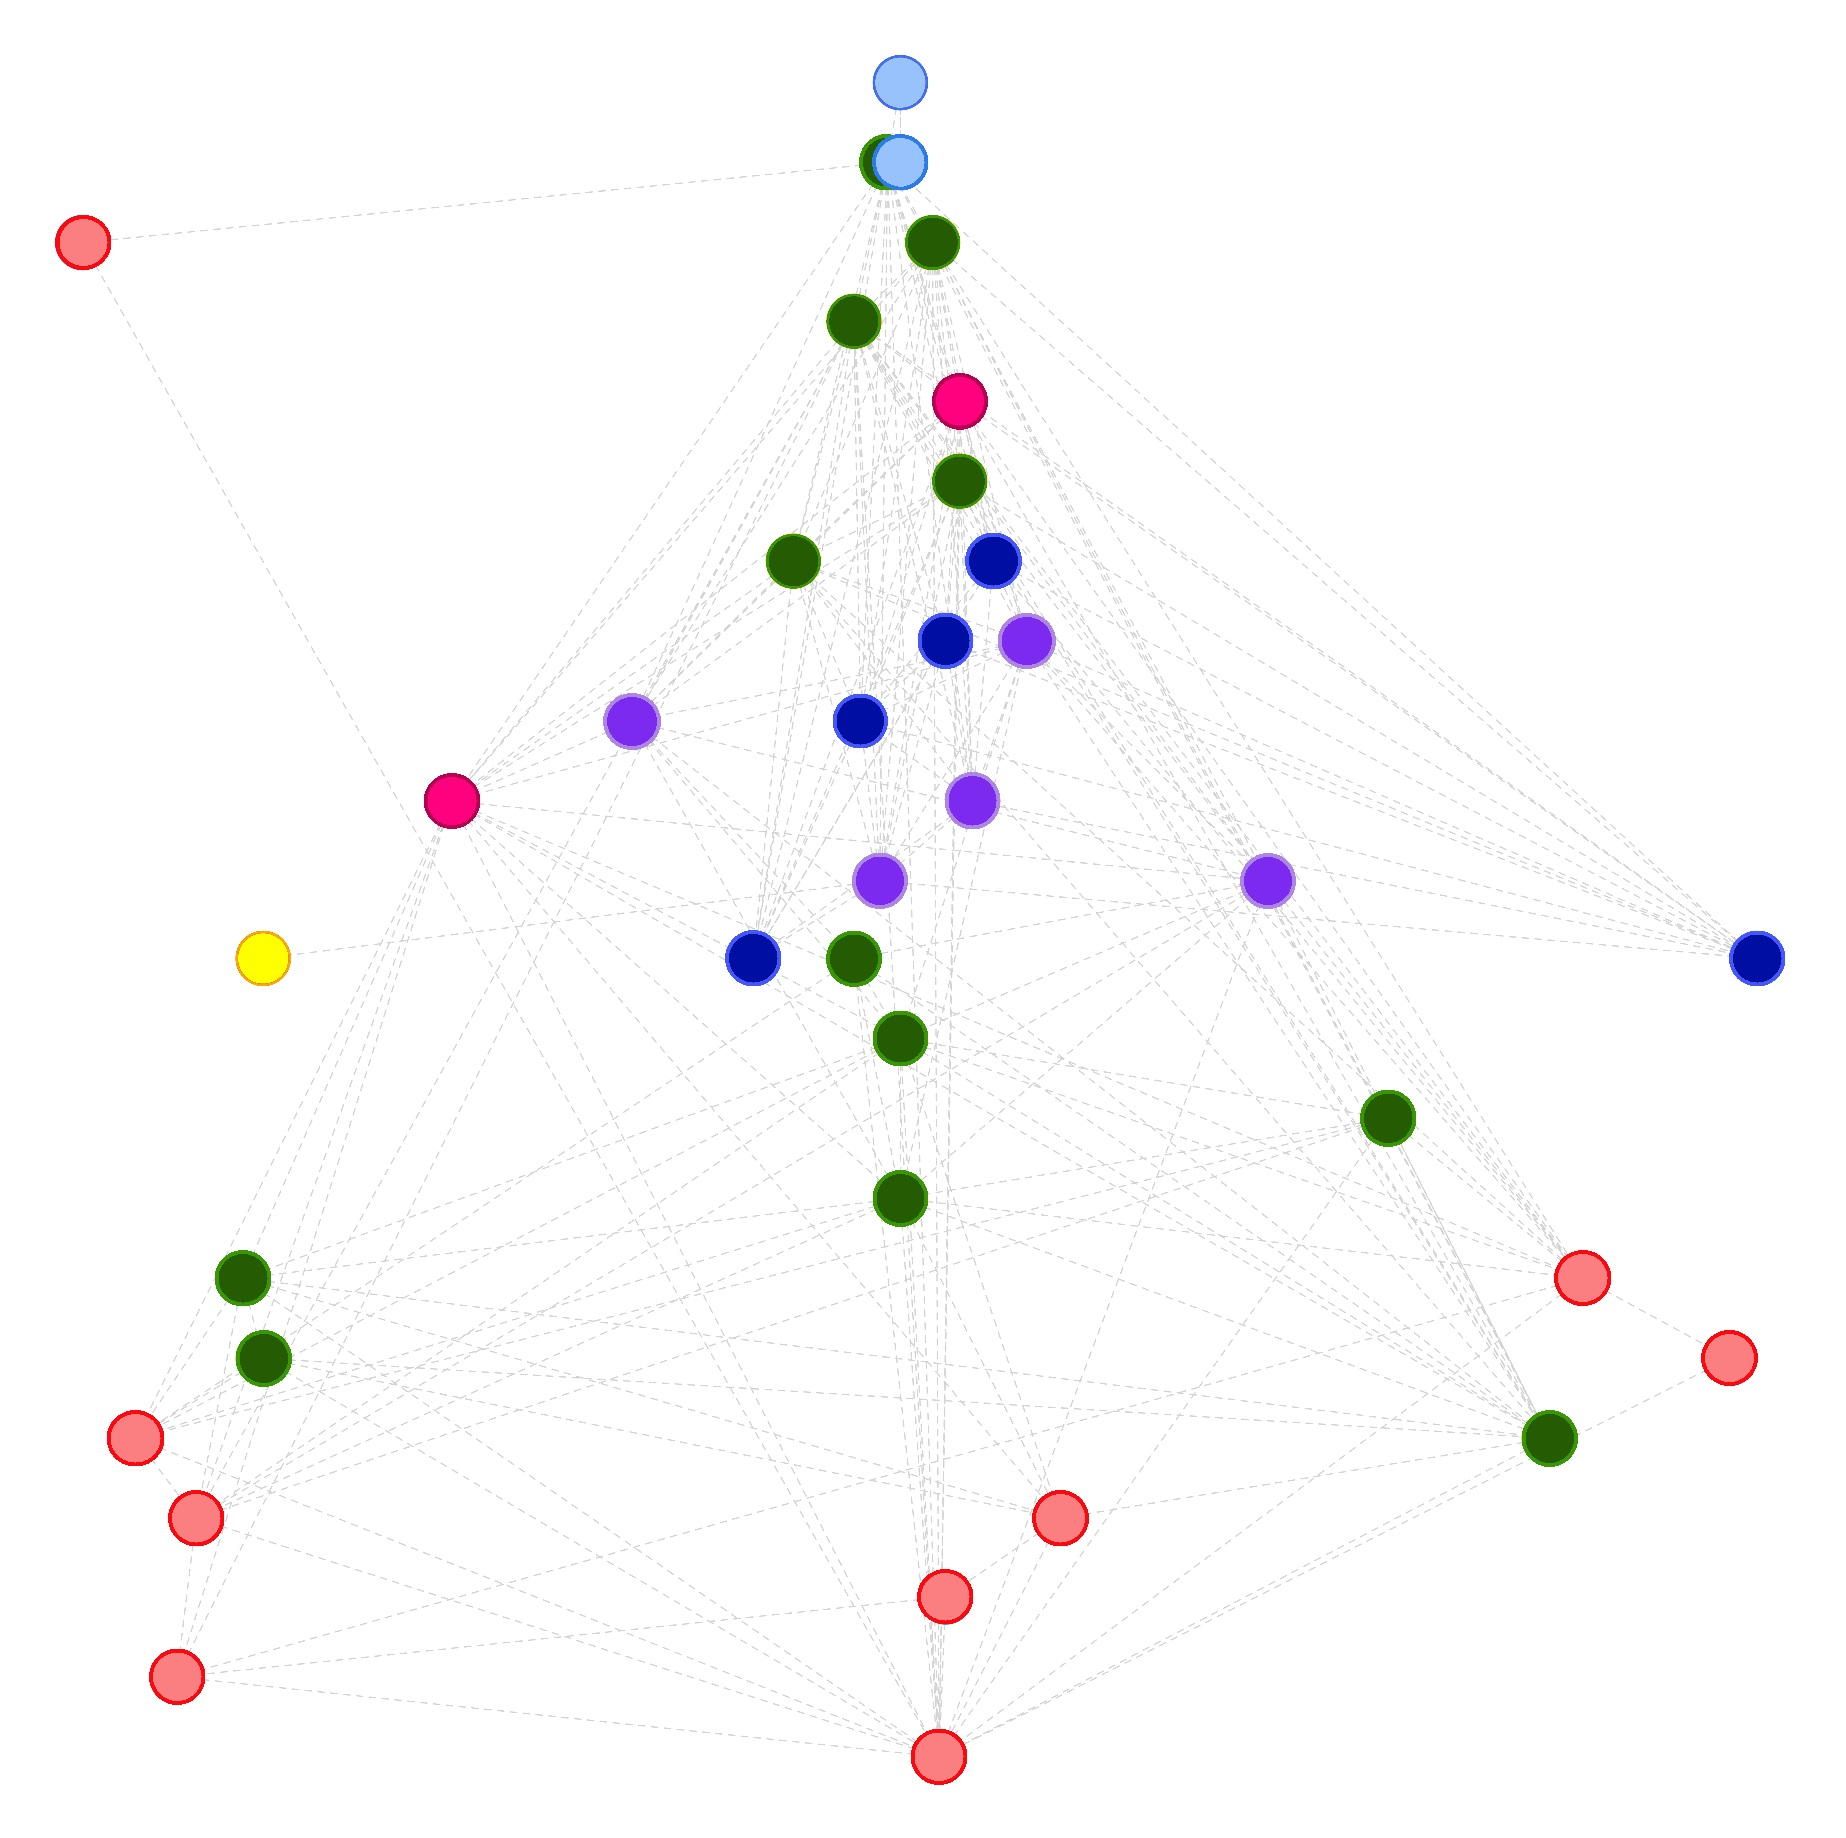
\includegraphics[height=0.35\textheight]{img/oot/module_hierarchical}
\caption{Sugiyama (hierarchical) layout (the direction of edges always
  points downwards, above \texttt{DEPENDS\_ON} below) of \textbf{modules} in the
  OOT Coq library. Modules are coloured according the most frequent (mode)
  colour of all definitions and proofs in it. Edges represent the
  \texttt{DEPENDS\_ON} relation between modules defined in
  Listing~\ref{lst:moddep}. This visually represents the chapter dependencies in
  BG and PF, starting with BG~1 at the bottom and ending with PF~14 (containing
  the actual proof of the Feit-Thompson OOT) at the top.}\label{fig:oot:modhier}
\end{figure}

Figures~\ref{fig:oot:hier} and~\ref{fig:oot:hierflip} show two extremes of how
one may approach the material. 

\begin{enumerate}
  \item Figure~\ref{fig:oot:hier} shows the hierarchical, Sugiyama layout. A
    consequence of this algorithm is that nodes are placed closest to their
    first use, usually done as a heuristic to minimise edge crossings.
    Intuitively, one can think of this approach as the lazy student who only
    studies a particular definition/proof \emph{just before} it is needed by
    some other part of the text (or like call-by-need evaluation in a non-strict
    programming language).  

  \item Figure~\ref{fig:oot:hierflip} shows that, swapping the direction of the
    edges does not simply flip the layout. In this vertically reflected image,
    nodes are placed \emph{lower/closest to the nodes using them}.  Intuitively,
    one can think of this approach as the eager student who studies \emph{any}
    definitions/proofs that will be required by \emph{any} later result \emph{as
    early as possible} (or like call-by-value evaluation in a programming
    language).  

\end{enumerate}

% Hierarchical
\begin{figure}[tp]
  \begin{minipage}{0.5\textwidth-0.5em}
    \centering
    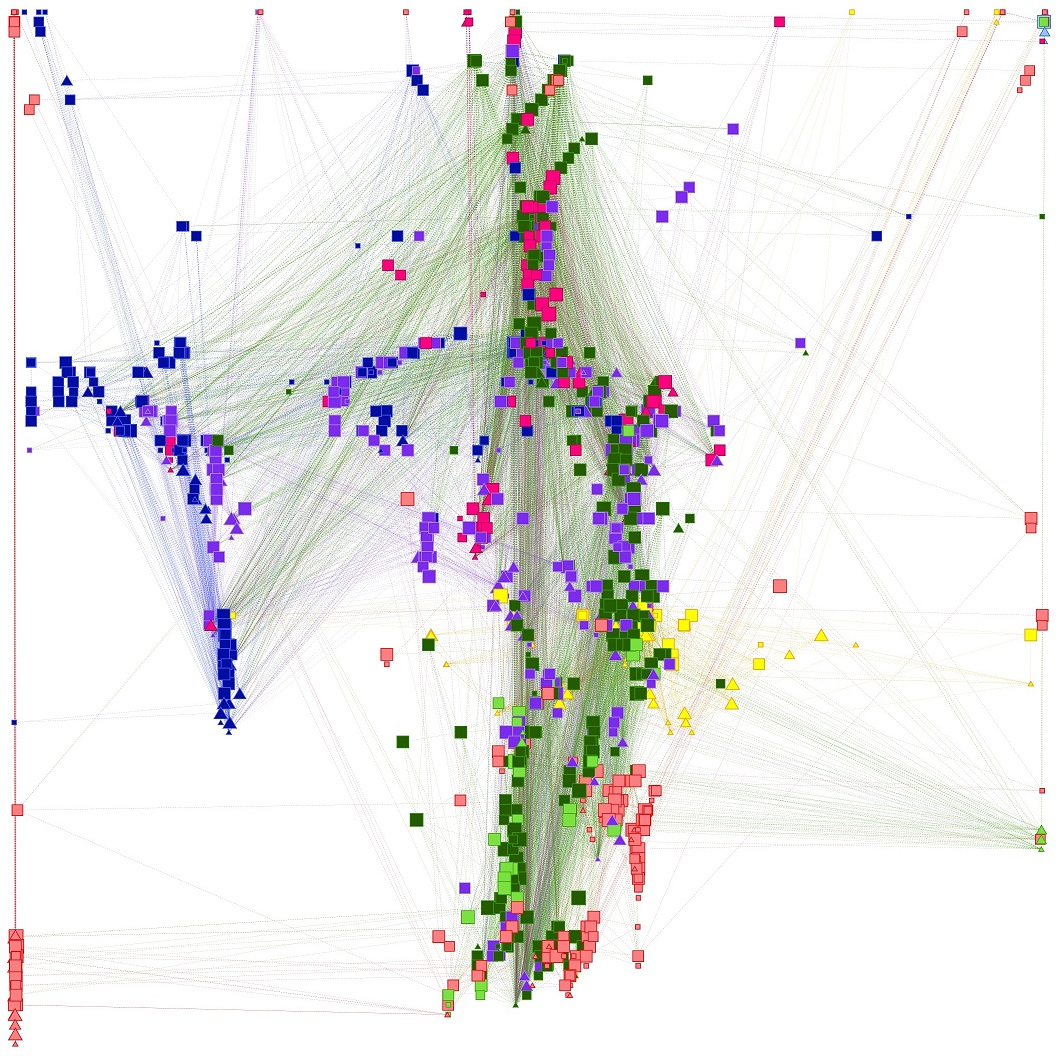
\includegraphics[width=\textwidth]{img/oot/hierarchical}
    \caption{Sugiyama (hierarchical) layout (the direction of edges point
      downwards) of \textbf{definitions and proofs} in the OOT Coq
      library. Colours are assigned by modularity clustering. Edges represent
      the \texttt{USES} relation: above \emph{uses} below. A by-product of
      this layout is that nodes are placed higher/closest to their
      \emph{users}.}\label{fig:oot:hier}
  \end{minipage}%
  \hspace{1em}%
  \begin{minipage}{0.5\textwidth-0.5em}
    \centering
		\reflectbox{\rotatebox[origin=c]{180}{%
			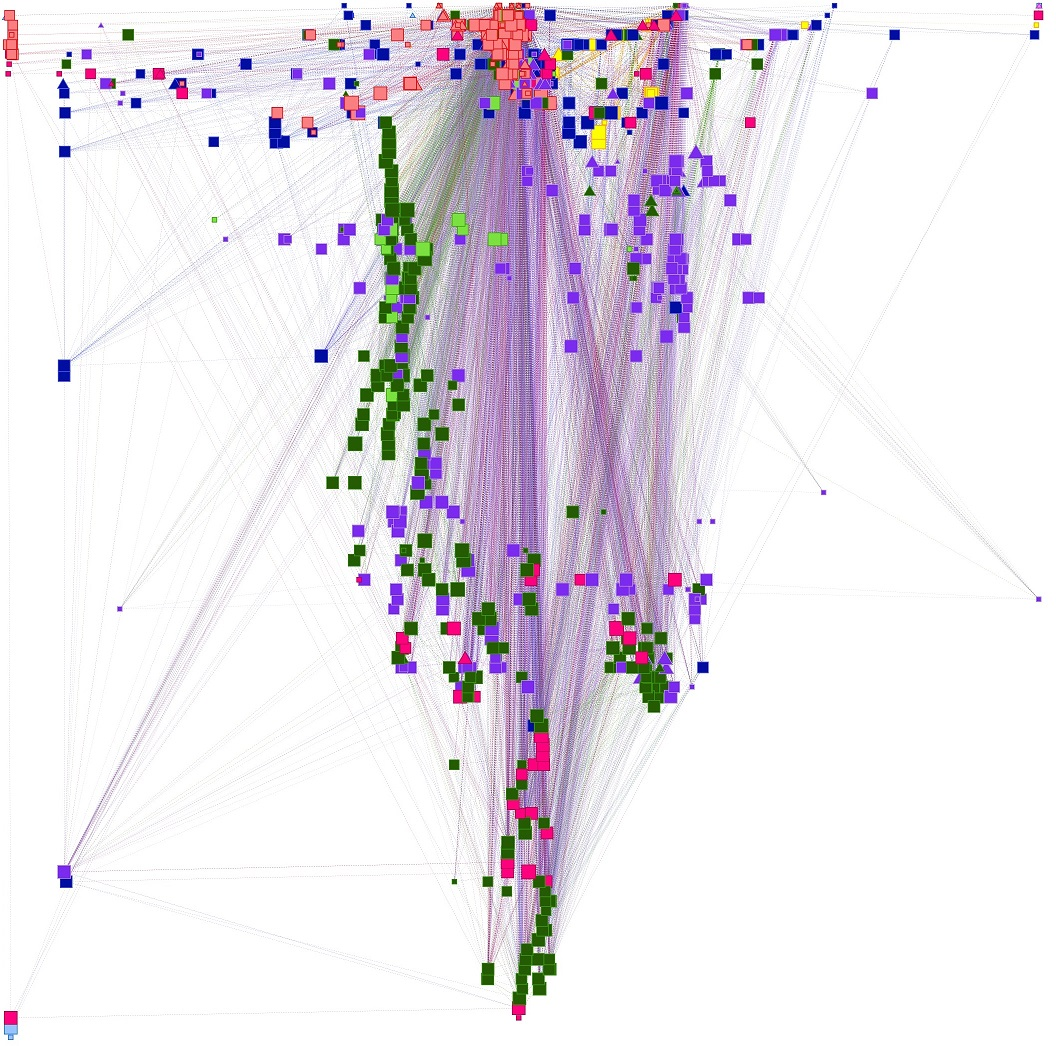
\includegraphics[width=\textwidth]{img/oot/hierarchical_flipped}}}
      \caption{Setup is the same as Figure~\ref{fig:oot:hierflip}, except that
      (a) the edge directions are \emph{reversed} and (b) the image is
      reflected vertically. It is still the case that above \emph{uses} below.
      However, doing this has the effect of placing a node lower/closest to
      the nodes \emph{using} it. An interpretation of this effect is provided
      in~\ref{subsubsec:oot:visual}~\nameref{subsubsec:oot:visual}.}\label{fig:oot:hierflip}
  \end{minipage}
\end{figure}

One could conjecture that Figure~\ref{fig:oot:hier} shows how mathematics is
developed (a narrow foundation, top-down refinement, creating proofs/definitions
as and when needed, several independent lines of thought) and
Figure~\ref{fig:oot:hierflip} shows how mathematics is presented (a broad base
of all the groundwork that will be needed first, followed by a bottom-up,
rapidly developing, linear argument which uses the base extensively). The
similarities between Figures~\ref{fig:oot:modhier} and~\ref{fig:oot:hierflip}
are evidence for this interpretation.

\section{Summary}

In this chapter, I evaluated how well my project had achieved its two major aims
(Section~\ref{intro:aims}).

\begin{enumerate} 

  \item To evaluate the first aim of choosing the correct model (as part of
    representing Coq libraries as Neo4j graph databases), I compared this
    project's features and performance against other, existing tools that aim to
    help a user understand a Coq library. 

    \begin{itemize}

      \item I showed that this project either supports, or can be extended to
        support, every feature supported by other tools. This project also
        supports additional features not in other tools: structural queries,
        network-analysis algorithms and visualisations.

      \item I showed that this project is slightly slower than other tools
        because it has more features and is more flexible.

    \end{itemize}

  \item To evaluate the second aim of analysing and highlighting the structure
    of Coq libraries, I examined this project's output on two examples:
    CoqRegExp (a small case) and OOT (a large case). It is not possible to gain
    the following insights using other tools.

    \begin{itemize}

      \item Analysing the output for CoqRegExp revealed the following insights:
        lemmas were the most common kind of proof-object; the definitions of a
        regular-expression and what it means for a regular-expression to match a
        string were the most important proof-objects (by PageRank values); each
        module and the library a whole is primarily split into two groups
        (\glblue{executable functions} and \gorange{proofs of correctness}); 

      \item Analysing the output for OOT revealed the following insights: there
        are many proof-objects in BG and PF that do not lead to the proof of the
        Feit-Thompson OOT (about 4-6 every section, most of them lemmas);
        clustering proof-objects shows grouping at the module-level; these
        groups demarcate different parts/phases of BG and PF; this phase
        demarcation is also reflected in the \emph{reversed dependencies} at the
        proof-object level; the differences obtained by reversing proof-object
        dependencies could be a visual representation of the difference between
        \emph{developing} mathematics (top-down, as needed) versus
        \emph{presenting} mathematics (bottom-up, eagerly).

    \end{itemize}

\end{enumerate}
